% !TeX root = ../../Report.tex
% !TeX encoding = UTF-8
در این پوشه به بانک اطلاعات پرداخته می‌شود و تمام اطلاعات از پایگاه داده واکشی می‌شود.

\begin{figure}[H]
	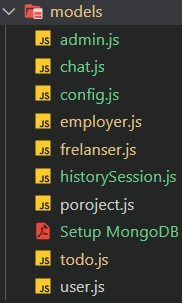
\includegraphics[width=.3\textwidth]{Folders-Files/models.png}
	\centering
	\caption{ساختار پوشه مدل}
	\label{fig:folder-models}
\end{figure}

\subsection{فایل user}
در این فایل به بانک اطلاعات برای ثبت اطلاعات کاربر از جمله مشخصات شناسنامه‌ای، اطلاعات کاربری و رمز و ... پرداخته شده است.

\paragraph{\rl{setUser}:}
ثبت اطلاعات کاربر.
\\
\textbf{توضیحات}
\hr
\begin{flushleft}
	\framebox[.9\textwidth][l]{
		\lr{
			\textcolor{type}{void}
			\textcolor{func}{setUser}
			\textcolor{symb}{(}
			\textcolor{type}{object}
			\textcolor{arg}{newUser}
			\textcolor{symb}{,}
			\textcolor{type}{object}
			\textcolor{arg}{callback}
			\textcolor{symb}{);}
		}
	}
\end{flushleft}
ثبت طلاعات کاربر در بانک اطلاعات.
\\
\textbf{پارامترها}
\hr \\[10pt]
\begin{tabular}{|m{4cm}|m{3cm}|m{10cm}|}
	\hline
	\multicolumn{1}{|c}{پارامتر}
	&
	\multicolumn{1}{|c}{نوع}
	&
	\multicolumn{1}{|c|}{توضیحات}
	\\
	\hline
	\multicolumn{1}{|c}{newUser}
	&
	\multicolumn{1}{|c|}{object}
	&
	0
	\\
	\hline
	\multicolumn{1}{|c}{callback}
	&
	\multicolumn{1}{|c|}{object}
	&
	0
	\\
	\hline
\end{tabular}
\\[10pt]
\textbf{خروجی}
\hr \\
در صورتی که ، در غیر این صورت .


\paragraph{\rl{getUserByEmail}:}
دریافت اطلاعات کاربر با پست الکترونیک.
\\
\textbf{توضیحات}
\hr
\begin{flushleft}
	\framebox[.9\textwidth][l]{
		\lr{
			\textcolor{type}{void}
			\textcolor{func}{getUserByEmail}
			\textcolor{symb}{(}
			\textcolor{type}{string}
			\textcolor{arg}{email}
			\textcolor{symb}{,}
			\textcolor{type}{object}
			\textcolor{arg}{callback}
			\textcolor{symb}{);}
		}
	}
\end{flushleft}
دریافت طلاعات کاربر از بانک اطلاعات توسط پست الکترونیک.
\\
\textbf{پارامترها}
\hr \\[10pt]
\begin{tabular}{|m{4cm}|m{3cm}|m{10cm}|}
	\hline
	\multicolumn{1}{|c}{پارامتر}
	&
	\multicolumn{1}{|c}{نوع}
	&
	\multicolumn{1}{|c|}{توضیحات}
	\\
	\hline
	\multicolumn{1}{|c}{email}
	&
	\multicolumn{1}{|c|}{string}
	&
	0
	\\
	\hline
	\multicolumn{1}{|c}{callback}
	&
	\multicolumn{1}{|c|}{object}
	&
	0
	\\
	\hline
\end{tabular}
\\[10pt]
\textbf{خروجی}
\hr \\
در صورتی که ، در غیر این صورت .


\paragraph{\rl{getUserById}:}
دریافت اطلاعات کاربر با ID.
\\
\textbf{توضیحات}
\hr
\begin{flushleft}
	\framebox[.9\textwidth][l]{
		\lr{
			\textcolor{type}{void}
			\textcolor{func}{getUserById}
			\textcolor{symb}{(}
			\textcolor{type}{int}
			\textcolor{arg}{id}
			\textcolor{symb}{,}
			\textcolor{type}{object}
			\textcolor{arg}{callback}
			\textcolor{symb}{);}
		}
	}
\end{flushleft}
دریافت طلاعات کاربر از بانک اطلاعات توسط ID.
\\
\textbf{پارامترها}
\hr \\[10pt]
\begin{tabular}{|m{4cm}|m{3cm}|m{10cm}|}
	\hline
	\multicolumn{1}{|c}{پارامتر}
	&
	\multicolumn{1}{|c}{نوع}
	&
	\multicolumn{1}{|c|}{توضیحات}
	\\
	\hline
	\multicolumn{1}{|c}{id}
	&
	\multicolumn{1}{|c|}{int}
	&
	0
	\\
	\hline
	\multicolumn{1}{|c}{callback}
	&
	\multicolumn{1}{|c|}{object}
	&
	0
	\\
	\hline
\end{tabular}
\\[10pt]
\textbf{خروجی}
\hr \\
در صورتی که ، در غیر این صورت .

\subsection{فایل employer}
در این فایل به بانک اطلاعات برای اطلاعات داشبورد کارفرما مانند ثبت و بروزرسانی پروژه، دریافت پیشنهادهای انجام پروژه و ... پرداخته شده است.

\subsection{فایل frelanser}
در این فایل به بانک اطلاعات برای ‌اطلاعات داشبورد فریلنسر مانند ثبت رزومه، ثبت پیشنهاد برای انجام پروژه و ... پرداخته شده است.
